\documentclass[a4paper, 11pt]{article}

\usepackage[utf8]{inputenc}
\usepackage{amsmath,amssymb}
\usepackage{epsfig}  
\usepackage{setspace}
\usepackage{graphicx}

\voffset -0cm
\hoffset 0.0cm
\textheight 22cm
\textwidth 16cm
\topmargin 0.0cm
\oddsidemargin 0.0cm
\evensidemargin 0.0cm


\title{\bf{TP5 \\ Connected Component Applications}}
\author{}
\date{}


%%%%%%%%%%%%%%%%%%%%%%%%%%%
%%% Debut du document %%%%%
%%%%%%%%%%%%%%%%%%%%%%%%%%%
\begin{document}
\maketitle

You must first finish the implementation of the connected components extraction viewed in TP4.

\section*{\bf Counting blobs}

The goal here is to count the number of blobs in the image blobs.pgm using the connected component algorithm.
Once you can identify each blob, compute their respective centroid and their volume (by counting the number of pixels).

If we suppose that a blob is an ellipse, can you compute its major and minor axis ?

\begin{figure}
  \centering
  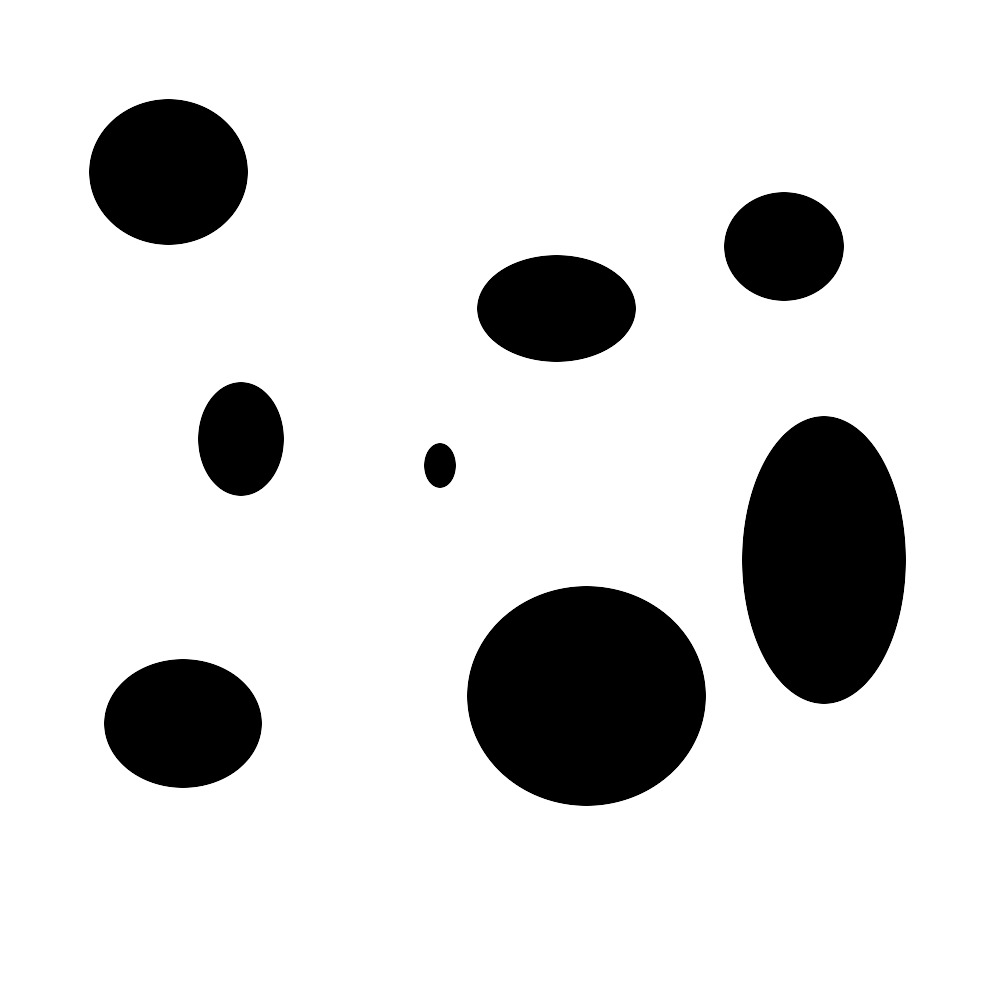
\includegraphics[width=0.5\textwidth]{blobs}
  \caption{An example of blobs}
\end{figure}

\section*{\bf Morphologic Dilatation and Erosion}

Morphology is a broad set of image processing operations that process images based on shapes. 
Morphological operations apply a structuring element to an input image, creating an output image of the same size. 
In a morphological operation, the value of each pixel in the output image is based on a comparison of the corresponding pixel in the input image with its neighbors. 

The most basic morphological operations are dilation and erosion. 
For each pixels $p$ in the input image, its value after dilation (resp. erosion) is the maximum (resp. minimum) value between all neighbor pixels defined by the mask.
More formally, let $P(p)$ be the value of the pixel $p$ in the input image. The dilation by a mask $\sigma$ denoted $P^{(\sigma)}$ of the input image is:
\[
  P^{(\sigma)}(p) = \max_{q\in\sigma(p)} P(q)
\]
and the erosion $P_{(\sigma)}$ is
\[
  P_{(\sigma)}(p) = \min_{q\in\sigma(p)} P(q).
\]

\paragraph{Question} Implement the two operations and test them using different masks.

\paragraph{Question} Use an operation of erosion to disconnect blobs in blobs2.pgm and then apply your connected component algorithm to count them.

\section*{\bf Morphologic Opening}

An opening is defined as an erosion followed by a dilation using the same structuring element for both operations.
The opening operator therefore requires two inputs: an image to be opened, and a structuring element.

\paragraph{Question} Use the opening operation to remove lines in art3.pgm

\paragraph{Question} Use the opening operation to isolate the big blobs in cell4.pgm and then count them.

\end{document}

